\section{Piecewise Constant Curvature Simulations}\label{sec:promasens:pcc_simulations}
We evaluate the proposed methodology for estimating the \gls{PCC} kinematic configuration $q \in \mathbb{R}^{3n_\mathrm{b}}$ of soft continuum robots thoroughly in simulations.
The PCC model allows for bending and elongation of each segment in 3D space. Please refer to Appendix~\ref{sub:promasens:kinematic_model_pcc} for more details.
We vary the number of robot segments $n_\mathrm{b}$, remove and add sensors (i.e. change $n_\mathrm{s}$), modify the arrangement of sensors, and the direction of the earth's magnetic field $n_\mathrm{e}$. 
To motivate some of the unique advantages of our method, we use the same learned neural network weights for all these trials.

\begin{landscape}
\begingroup
\setlength{\tabcolsep}{2pt} % Default value: 6pt
\begin{table*}[hbt]
\centering
\caption{
Simulation results: First, we report the absolute Root Mean-Squared Error (RMSE) $e_{u}$ of sensor measurement predictions on the test set averaged across all sensors on the robot. Next, we state the relative RMSE [\%] of each robot configuration estimate. All results are trained on a trajectory with randomly sampled configurations and sensor kinematic parameters for each segment separately and evaluated on a lemniscate trajectory.
The first section applies our methodology to robots consisting of a different number of segments $n_\mathrm{b}$ with three sensors attached to the tip of each segment.
The number of sensors is varied in the second section for a three-segment robot with all sensors placed symmetrically. 
The third set of trials then investigates how robust the method is to change the kinematic parameters of the sensors, such as the tilting angle of the sensors $\psi_\mathrm{s}$ and the radial distance of the sensors $d_{\mathrm{s},\mathrm{r}}$.
Finally, we apply the earth's magnetic field along different cardinal directions in the inertial frame.
The RMSE of the configuration estimates is normalized with the range of the dataset for each configuration variable as stated in \eqref{eq:promasens:relative_RMSE}. We report the error as $\text{mean} \pm \text{stdev}$ and compute the statistics over three different random seeds. The random seed determines at the start of the training the initialization of the neural network weights.
}
% \begin{tabular}{l r rrr rrr rrr}\toprule
% \textbf{Simulation} & $e_{u}$ [mT] & $e_{\Delta_{x,1}}$ [\%] & $e_{\Delta_{y,1}}$ [\%] & $e_{\delta L_1}$ [\%] & $e_{\Delta_{x,2}}$ [\%] & $e_{\Delta_{y,2}}$ [\%] & $e_{\delta L_2}$ [\%] & $e_{\Delta_{x,3}}$ [\%] & $e_{\Delta_{y,3}}$ [\%] & $e_{\delta L_3}$ [\%]\\
% \midrule
% \# of segments: $n_\mathrm{b} = 1$ & $1.5 \pm 0.2$ & $1.7 \pm 1.0$ & $1.8 \pm 1.1$ & $2.8 \pm 0.6$ & - & - & - & - & - & -\\
% \# of segments: $n_\mathrm{b} = 2$ & $1.5 \pm 0.1$ & $4.2 \pm 1.3$ & $3.9 \pm 0.6$ & $6.3 \pm 1.3$ & $2.3 \pm 0.6$ & $2.2 \pm 0.3$ & $4.1 \pm 1.3$ & - & - & -\\
% \# of segments: $n_\mathrm{b} = 3$ & $1.5 \pm 0.2$ & $3.7 \pm 2.1$ & $4.7 \pm 1.6$ & $6.0 \pm 2.0$ & $2.6 \pm 1.6$ & $2.5 \pm 1.5$ & $5.5 \pm 1.6$ & $1.6 \pm 1.2$ & $1.6 \pm 1.1$ & $2.7 \pm 1.4$\\
% \midrule
% \# of sensors: $n_\mathrm{s} = 6$ & $1.5 \pm 0.2$ & $3.9 \pm 1.2$ & $24.4 \pm 2.7$ & $8.4 \pm 2.6$ & $2.5 \pm 1.3$ & $53.2 \pm 5.0$ & $6.0 \pm 1.7$ & $1.5 \pm 1.1$ & $52.3 \pm 7.3$ & $3.1 \pm 1.0$\\
% \# of sensors: $n_\mathrm{s} = 9$ & $1.5 \pm 0.2$ & $3.7 \pm 2.1$ & $4.7 \pm 1.6$ & $6.0 \pm 2.0$ & $2.6 \pm 1.6$ & $2.5 \pm 1.5$ & $5.5 \pm 1.6$ & $1.6 \pm 1.2$ & $1.6 \pm 1.1$ & $2.7 \pm 1.4$\\
% \# of sensors: $n_\mathrm{s} = 12$ & $1.5 \pm 0.1$ & $3.7 \pm 1.6$ & $3.9 \pm 1.3$ & $4.6 \pm 2.4$ & $2.6 \pm 1.3$ & $2.6 \pm 1.2$ & $4.4 \pm 1.9$ & $1.6 \pm 1.2$ & $1.5 \pm 1.3$ & $2.5 \pm 1.6$\\
% \# of sensors: $n_\mathrm{s} = 18$ & $1.6 \pm 0.2$ & $3.2 \pm 1.5$ & $3.5 \pm 1.3$ & $4.2 \pm 1.8$ & $2.4 \pm 1.3$ & $2.5 \pm 1.2$ & $4.4 \pm 1.8$ & $1.5 \pm 1.3$ & $1.3 \pm 1.1$ & $2.5 \pm 1.5$\\
% \midrule
% nominal & $1.5 \pm 0.2$ & $3.7 \pm 2.1$ & $4.7 \pm 1.6$ & $6.0 \pm 2.0$ & $2.6 \pm 1.6$ & $2.5 \pm 1.5$ & $5.5 \pm 1.6$ & $1.6 \pm 1.2$ & $1.6 \pm 1.1$ & $2.7 \pm 1.4$\\
% sensors tilted: $\psi_\mathrm{s} = \SI{10}{\degree}$ & $1.5 \pm 0.2$ & $8.1 \pm 4.0$ & $6.4 \pm 2.0$ & $4.7 \pm 0.7$ & $5.1 \pm 2.3$ & $3.8 \pm 0.8$ & $5.6 \pm 2.4$ & $2.8 \pm 1.2$ & $1.9 \pm 0.8$ & $4.1 \pm 0.6$\\
% $d_{\mathrm{s},\mathrm{r}} = \SI{16}{mm}, \psi_\mathrm{s} = \SI{10}{\degree}$ & $1.5 \pm 0.1$ & $4.0 \pm 2.1$ & $4.3 \pm 1.6$ & $4.6 \pm 1.3$ & $2.9 \pm 0.3$ & $2.4 \pm 0.3$ & $5.2 \pm 1.6$ & $1.6 \pm 1.0$ & $1.6 \pm 0.8$ & $3.1 \pm 1.0$ \\
% % \midrule
% % FEM nominal & $0.0 \pm 0.0$ & $0.0 \pm 0.0$ & $0.0 \pm 0.0$ & $0.0 \pm 0.0$ & $0.0 \pm 0.0$ & $0.0 \pm 0.0$ & $0.0 \pm 0.0$ & $0.0 \pm 0.0$ & $0.0 \pm 0.0$ & $0.0 \pm 0.0$\\
% \bottomrule
% \end{tabular}

\begin{tabular}{cl r rrr rrr rrr}\toprule
\textbf{Simulation} & \textbf{Specifications} & $e_{u}$ [mT] & $e_{\Delta_{x,1}}$ [\%] & $e_{\Delta_{y,1}}$ [\%] & $e_{\delta L_1}$ [\%] & $e_{\Delta_{x,2}}$ [\%] & $e_{\Delta_{y,2}}$ [\%] & $e_{\delta L_2}$ [\%] & $e_{\Delta_{x,3}}$ [\%] & $e_{\Delta_{y,3}}$ [\%] & $e_{\delta L_3}$ [\%]\\
\midrule
\multirow{3}{*}{\makecell{Variation of\\ \# of segments}} & $n_\mathrm{b}$=1, $n_\mathrm{s}$=3 & $0.015 \pm 0.002$ & $1.7 \pm 1.0$ & $1.8 \pm 1.1$ & $2.8 \pm 0.6$ & - & - & - & - & - & -\\
& $n_\mathrm{b}$=2, $n_\mathrm{s}$=6 & $0.015 \pm 0.001$ & $4.2 \pm 1.3$ & $3.9 \pm 0.6$ & $6.3 \pm 1.3$ & $2.3 \pm 0.6$ & $2.2 \pm 0.3$ & $4.1 \pm 1.3$ & - & - & -\\
& $n_\mathrm{b}$=3, $n_\mathrm{s}$=9 & $0.015 \pm 0.002$ & $3.7 \pm 2.1$ & $4.7 \pm 1.6$ & $6.0 \pm 2.0$ & $2.6 \pm 1.6$ & $2.5 \pm 1.5$ & $5.5 \pm 1.6$ & $1.6 \pm 1.2$ & $1.6 \pm 1.1$ & $2.7 \pm 1.4$\\
\midrule
\multirow{4}{*}{\makecell{Variation of\\ \# of sensors}} &$n_\mathrm{b}$=3, $n_\mathrm{s}$=6 & $0.015 \pm 0.002$ & $3.9 \pm 1.2$ & $24.4 \pm 2.7$ & $8.4 \pm 2.6$ & $2.5 \pm 1.3$ & $53.2 \pm 5.0$ & $6.0 \pm 1.7$ & $1.5 \pm 1.1$ & $52.3 \pm 7.3$ & $3.1 \pm 1.0$\\
&$n_\mathrm{b}$=3, $n_\mathrm{s}$=9 & $0.015 \pm 0.002$ & $3.7 \pm 2.1$ & $4.7 \pm 1.6$ & $6.0 \pm 2.0$ & $2.6 \pm 1.6$ & $2.5 \pm 1.5$ & $5.5 \pm 1.6$ & $1.6 \pm 1.2$ & $1.6 \pm 1.1$ & $2.7 \pm 1.4$\\
&$n_\mathrm{b}$=3, $n_\mathrm{s}$=12 & $0.015 \pm 0.001$ & $3.7 \pm 1.6$ & $3.9 \pm 1.3$ & $4.6 \pm 2.4$ & $2.6 \pm 1.3$ & $2.6 \pm 1.2$ & $4.4 \pm 1.9$ & $1.6 \pm 1.2$ & $1.5 \pm 1.3$ & $2.5 \pm 1.6$\\
&$n_\mathrm{b}$=3, $n_\mathrm{s}$=18 & $0.016 \pm 0.002$ & $3.2 \pm 1.5$ & $3.5 \pm 1.3$ & $4.2 \pm 1.8$ & $2.4 \pm 1.3$ & $2.5 \pm 1.2$ & $4.4 \pm 1.8$ & $1.5 \pm 1.3$ & $1.3 \pm 1.1$ & $2.5 \pm 1.5$\\
\midrule
Nominal & $n_\mathrm{b}$=3, $n_\mathrm{s}$= 9 & $0.015 \pm 0.002$ & $3.7 \pm 2.1$ & $4.7 \pm 1.6$ & $6.0 \pm 2.0$ & $2.6 \pm 1.6$ & $2.5 \pm 1.5$ & $5.5 \pm 1.6$ & $1.6 \pm 1.2$ & $1.6 \pm 1.1$ & $2.7 \pm 1.4$\\
Sensors tilted & $\psi_\mathrm{s}$=\SI{10}{\degree} & $0.015 \pm 0.002$ & $8.1 \pm 4.0$ & $6.4 \pm 2.0$ & $4.7 \pm 0.7$ & $5.1 \pm 2.3$ & $3.8 \pm 0.8$ & $5.6 \pm 2.4$ & $2.8 \pm 1.2$ & $1.9 \pm 0.8$ & $4.1 \pm 0.6$\\
Sensors shifted & $d_{\mathrm{s},\mathrm{r}}$=\SI{16}{mm} & $0.017 \pm 0.003$ & $3.4 \pm 1.5$ & $4.0 \pm 1.3$ & $6.2 \pm 2.5$ & $2.6 \pm 1.0$ & $2.8 \pm 1.8$ & $6.7 \pm 0.9$ & $1.6 \pm 1.2$ & $1.6 \pm 1.0$ & $4.0 \pm 2.0$ \\
\midrule
\multirow{3}{*}{\makecell{Earth\\ magnetic\\ field}} & $n_\mathrm{e}$=$(1,0,0)$ & $0.012 \pm 0.002$ & $2.0 \pm 0.4$ & $2.4 \pm 1.1$ & $4.3 \pm 1.3$ & $1.8 \pm 0.7$ & $1.9 \pm 0.3$ & $3.6 \pm 2.0$ & $1.5 \pm 0.3$ & $1.6 \pm 0.4$ & $3.2 \pm 0.9$\\
& $n_\mathrm{e}$=$(0,1,0)$ & $0.012 \pm 0.002$ & $1.9 \pm 0.5$ & $2.5 \pm 0.8$ & $3.8 \pm 1.1$ & $1.9 \pm 0.5$ & $2.0 \pm 0.2$ & $3.4 \pm 1.6$ & $1.5 \pm 0.3$ & $1.6 \pm 0.4$ & $3.3 \pm 0.8$\\
& $n_\mathrm{e}$=$(0,0,1)$ & $0.012 \pm 0.001$ & $2.0 \pm 0.7$ & $2.6 \pm 0.9$ & $4.1 \pm 0.9$ & $1.6 \pm 0.3$ & $1.7 \pm 0.3$ & $4.9 \pm 1.5$ & $1.5 \pm 0.5$ & $1.4 \pm 0.1$ & $3.9 \pm 0.3$\\
% \midrule
% FEM nominal & $0.0 \pm 0.0$ & $0.0 \pm 0.0$ & $0.0 \pm 0.0$ & $0.0 \pm 0.0$ & $0.0 \pm 0.0$ & $0.0 \pm 0.0$ & $0.0 \pm 0.0$ & $0.0 \pm 0.0$ & $0.0 \pm 0.0$ & $0.0 \pm 0.0$\\
\bottomrule
\end{tabular}
\label{tab:results_pcc_simulations}
\end{table*}
\endgroup
\end{landscape}

\begin{figure*}[hbt]
\centering
    \subfigure[Magnetic field for a three-segment robot]{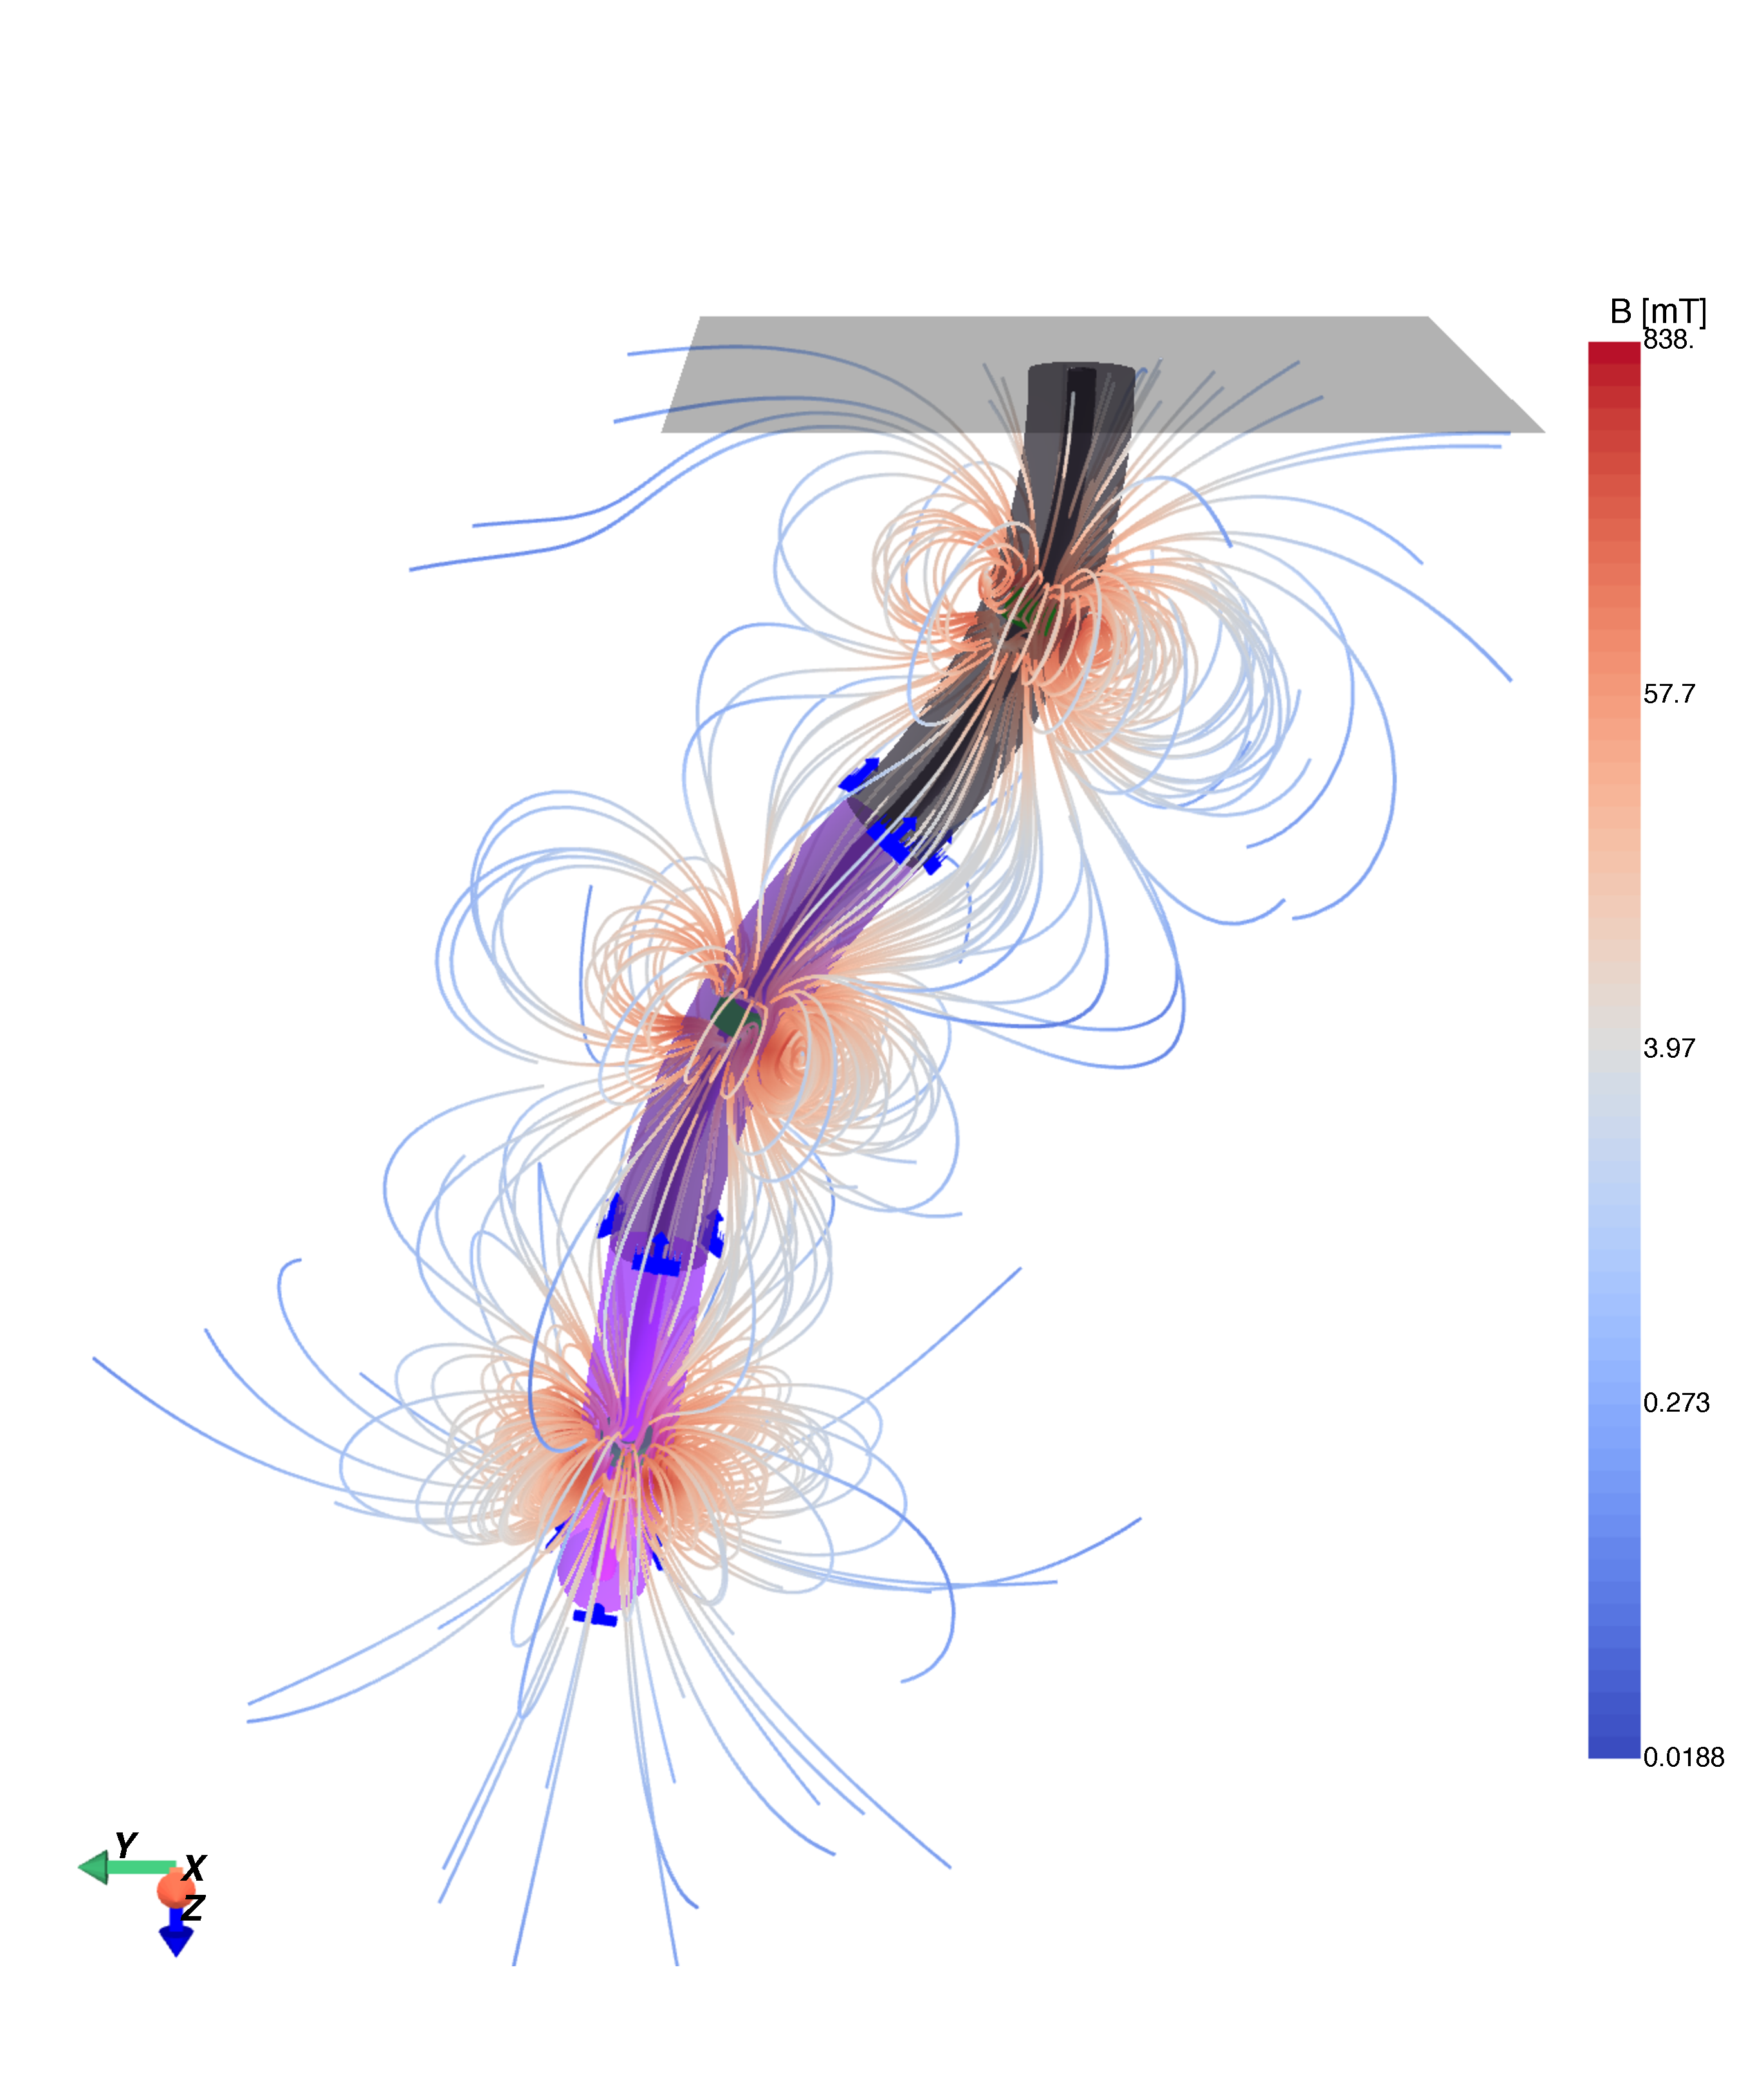
\includegraphics[width=0.3\textwidth]{promasens/figures/simulation_setup/analytical_simulation_three_segment_v2_cropped.pdf}}
    \subfigure[Simulated sensor failure]{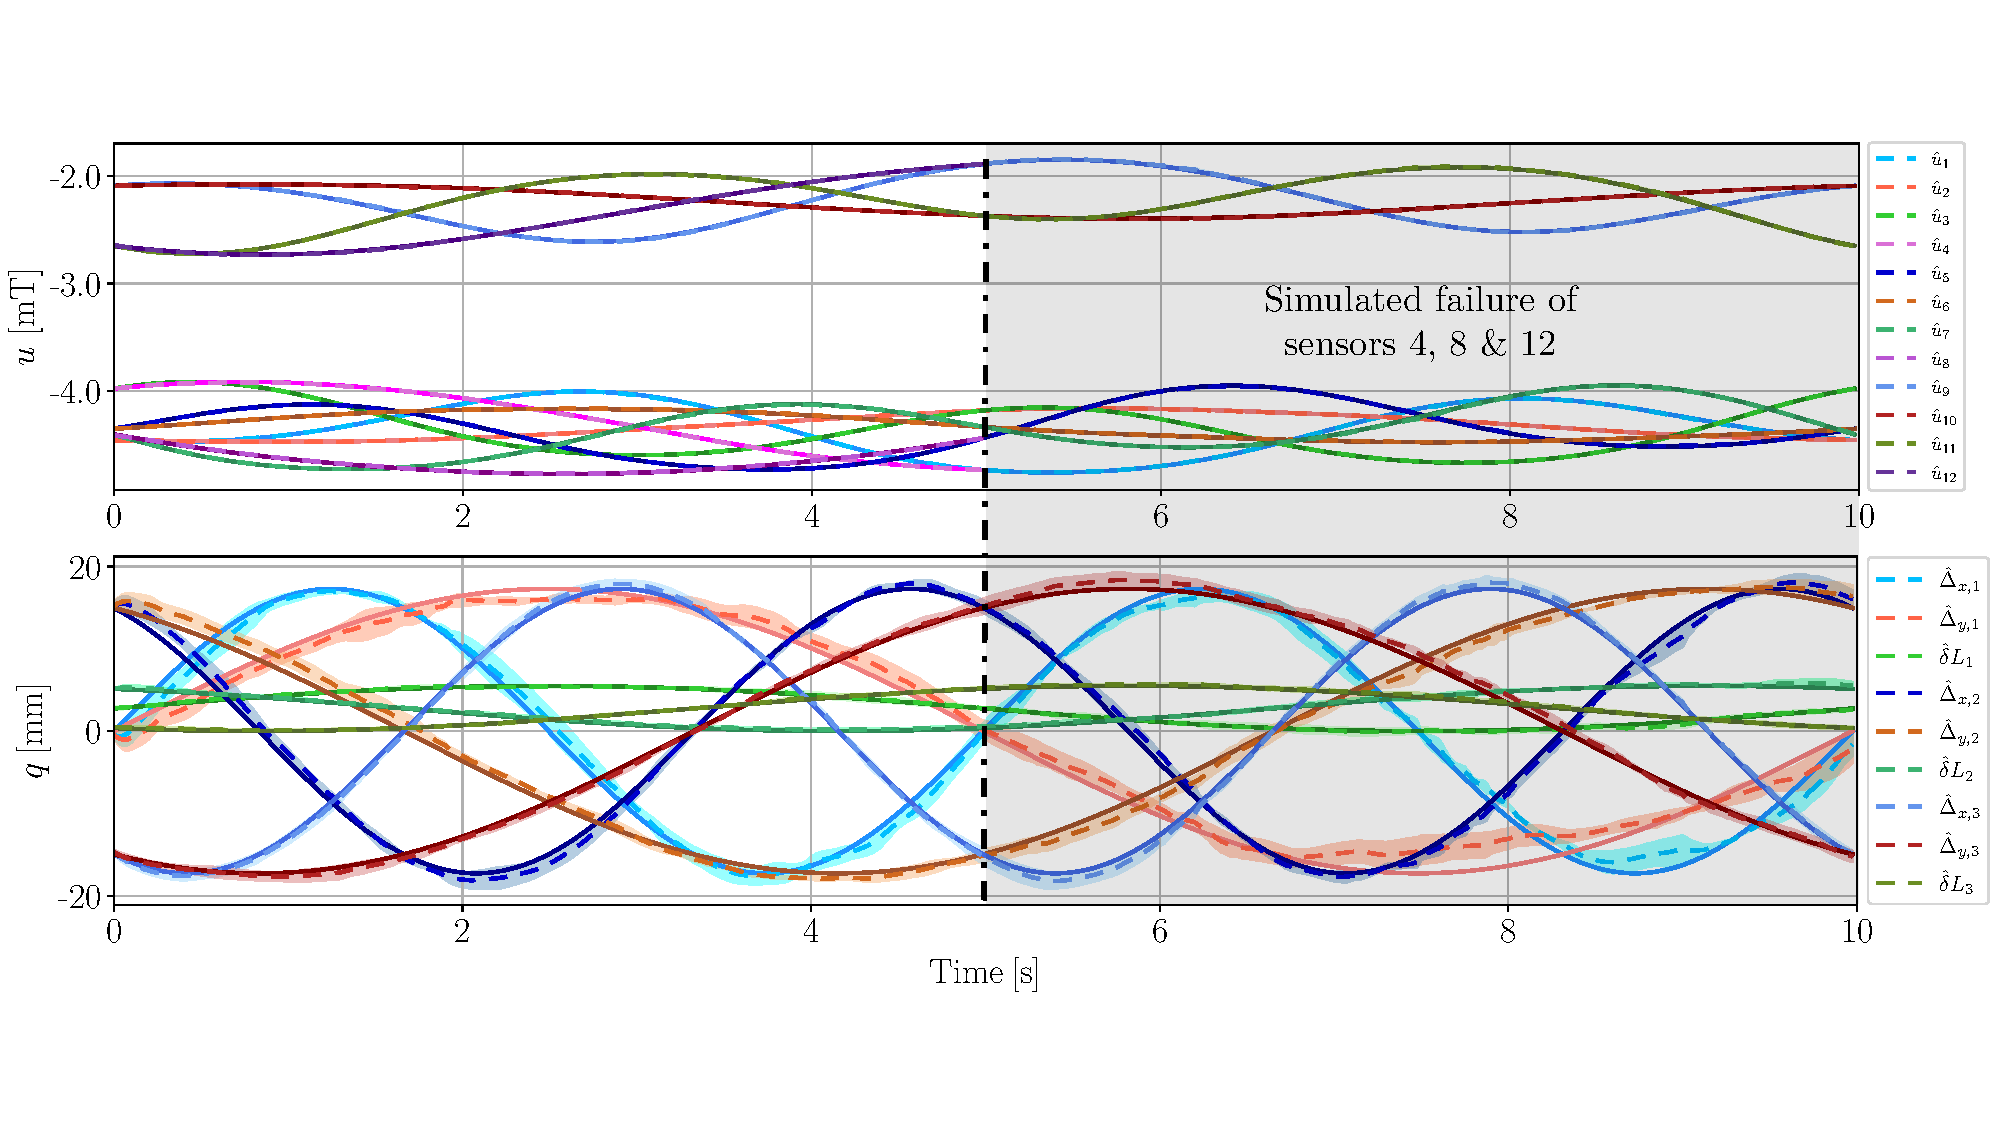
\includegraphics[width=0.68\textwidth]{promasens/figures/simulation_results/pcc/simulated_sensor_failure_cropped.pdf}\label{fig:promasens:simulated_sensor_failure}}
\caption{\textbf{Panel (a):} Simulated magnetic field of a robot with three segments. The blue arrows mark the measurement directions of the sensors, the magnets are rendered in green and the three segments are visualized in a color sequence from black to violet. The magnetic flux density $B$ is shown via streamlines and logarithmic coloring. \textbf{Panel (b)}: Sensor measurement predictions (top) and configuration estimates (bottom) for a three-segment robot with twelve sensors nominally. We simulate a sensor failure of the 4th, 8th, and 12th sensors after \SI{5}{s} of trajectory time by removing the measurements of these sensors from the gradient descent. This can be compensated automatically by the redundancy of the sensor configuration. We plot the ground-truth values $u$ and $q$ in solid, the estimate $\hat{u}$ and $\hat{q}$ as a mean over three random seeds with dashed lines and the standard deviation as an error band.}
\end{figure*}

\subsection{Simulation setup}\label{sub:promasens:pcc_simulations:simulation_setup}
In our simulations, we consider a robot consisting of one, two, or three segments. % which all behave according to the Constant Curvature (CC) assumption and can also elongate~\citep{della2020improved}. 
All cylindrical segments have an unextended length of $L_{0,i} = \SI{110}{mm}$ and a radius of $d_i = \SI{22}{mm}$. Each segment has a neodymium N50 ring magnet of outer diameter \SI{12}{mm}, inner diameter \SI{6}{mm} and thickness \SI{6}{mm} integrated along the backbone at a distance of $d_{\mathrm{m}_k} = \SI{55}{mm}$ from the base of the segment.
In the nominal case, three sensors are placed symmetrically in the tip plane of each segment at a radius of \SI{13}{mm} from the center with the sensor measurement direction pointing along the local, negative z-axis of the tip plane $\{S_i\}$. We also consider alternative placements of the sensors, which we further detail in Section~\ref{sub:promasens:simulation_pcc_results}.

% \subsection{Magnetic field simulation}
% The crucial component of our simulation is the prediction of the magnetic field and corresponding sensor measurements for a given pose of the magnets.
% For this, we leverage Magpylib~\citep{magpylib2020}, a Python package for computing 3D static magnetic fields using analytical solutions.
We build on Magpylib~\citep{magpylib2020} to simulate the magnetic field behavior.
We model the magnets as cylindrical neodymium grade N50 rings with a magnetization of \SI{1450}{mT} in the local z-direction. 
After simulating the magnetic field, we rotate the B-field into the local reference frame of each sensor and take the local z-component of the magnetic flux density as the sensor measurement.
%Additionally, we add a static B-field representing the earth's magnetic field influence along the inertial x-axis and a magnitude of \SI{65}{\micro T}. To simulate the sensor measurements, we take into account the component of the B-field pointing along the local z-axis of the sensor.

% \subsection{Magnetic field simulation \textcolor{orange}{FEM}}
% We build on Netgen / NGSolve~\citep{netgen_ngsolve} to simulate the magnetic field behavior using \gls{FEM} by implementing the magnetostatic Maxwell equations.
% We model a cylindrical Neodymium grade N50 ring magnet with a magnetization of $M=(0,0,\SI{1.45}{T})^\mathrm{T}$ in local z-direction and a relative permeability of $\mu_r = 1.05$. 
% % Additionally, we add a static B-field representing the earth's magnetic field influence along the inertial x-axis and a magnitude of \SI{65}{\micro T}. To simulate the sensor measurements, we take into account the component of the B-field pointing along the local z-axis of the sensor.
% The remaining part of the control volume
% We mesh the magnets and the air with a maximum mesh size of \SI{6}{mm} and \SI{220}{mm} respectively.
% After solving the finite element problem, we rotate the B-field into the local reference frame for each sensor and take the z-component of the magnetic flux density as the sensor measurement.
%

\subsection{Prediction network}\label{sub:promasens:pcc_simulations:neural_network}
The training set consists of \SI{120000}{} random configurations sampled from uniform distribution $\Delta_{x,i} \sim \mathcal{U}(-\SI{20.7}{mm}, \SI{20.7}{mm})$, $\Delta_{y,i} \sim \mathcal{U}(-\SI{20.7}{mm}, \SI{20.7}{mm})$, and $\delta L_i \sim \mathcal{U}(0, \SI{5.5}{mm})$, where the upper bound represents a bending of the tip of \SI{54}{\degree} with respect to the base of a segment and an elongation of \SI{5}{\percent}. We also randomize the placement of the sensors in the training set. While in the nominal case, the first of the symmetrically placed sensors is placed on the local x-axis, we randomly sample an offset angle $\varphi_\mathrm{off} \sim \mathcal{U}(0, \frac{2\pi}{n_{\mathrm{s}_i}})$ for each training sample, where $n_{\mathrm{s}_i} = 3$ is the number of sensors per segment.
Finally, we also randomly sample the radial displacement of the sensors from the center with $d_{\mathrm{s}, \mathrm{r}} \sim \mathcal{U}(8.7, 17.3) \mathrm{mm}$ and consider a tilting of the sensors (e.g. a rotation around the tangential axis) with $\psi_\mathrm{s} \sim \mathcal{U}(\SI{-20}{\degree}, \SI{20}{\degree})$.
Before training, we randomly split off \SI{30}{\percent} of the training set for validation purposes.

We conducted a selection study involving hyperparameters and feed-forward neural network architectures (number of layers, nodes, and nonlinear activation layer types) on the validation set. % to select our training procedure for the sensor measurement prediction network. 
In particular, we aimed to generate a smooth loss landscape to improve the gradient descent convergence leading us to employ a Stochastic Gradient Descent (SGD) % ~\citep{ruder2016overview} 
optimizer in conjunction with the Stochastic Weight Averaging (SWA)~\citep{izmailov2018averaging} strategy.
The neural network itself %as depicted in Figure~\ref{fig:promasens:NNgradientdescent}
has $18$ layers in total and contains, after an initial 1D batch norm layer, four blocks and is concluded with a fully-connected layer at the end. Each block consists of a dropout with a probability of \SI{1}{\percent}, a linear layer, a ReLU, and a 1D batch norm layer. The hidden state is first increased to $96$ nodes, then to $256$ nodes, and finally reduced again to $64$ and $24$ nodes.
We minimize a Mean Squared Error (MSE) loss of the neural network prediction $\hat{u}_j(t)$ for $250$ epochs with batch size $650$ while setting an initial learning rate of $0.18$ for the cosine annealing learning rate scheduler~\citep{loshchilov2016sgdr}. The SWA~\citep{izmailov2018averaging} strategy is started after $125$ epochs.
% We train a neural network $f_{\pi_i}(\xi_j)$ for all sensors in each segment $i$.
We train the neural network such that all sensors in the $i^\mathrm{th}$ segment share the same weights $\pi_i$.
% The reason for this is that the sensors in the distal segment measure much lower magnetic field magnitudes than the sensors in the other segments as they are only influenced by one magnet (e.g. the magnet in the distal segment) resulting in poor convergence behavior when trained jointly on all segments.
When the training is finished, we select the model from the epoch with the lowest validation loss and save it for later testing.

\begin{figure*}[hbt]
  \centering
  \subfigure[$t=\SI{0}{s}$]{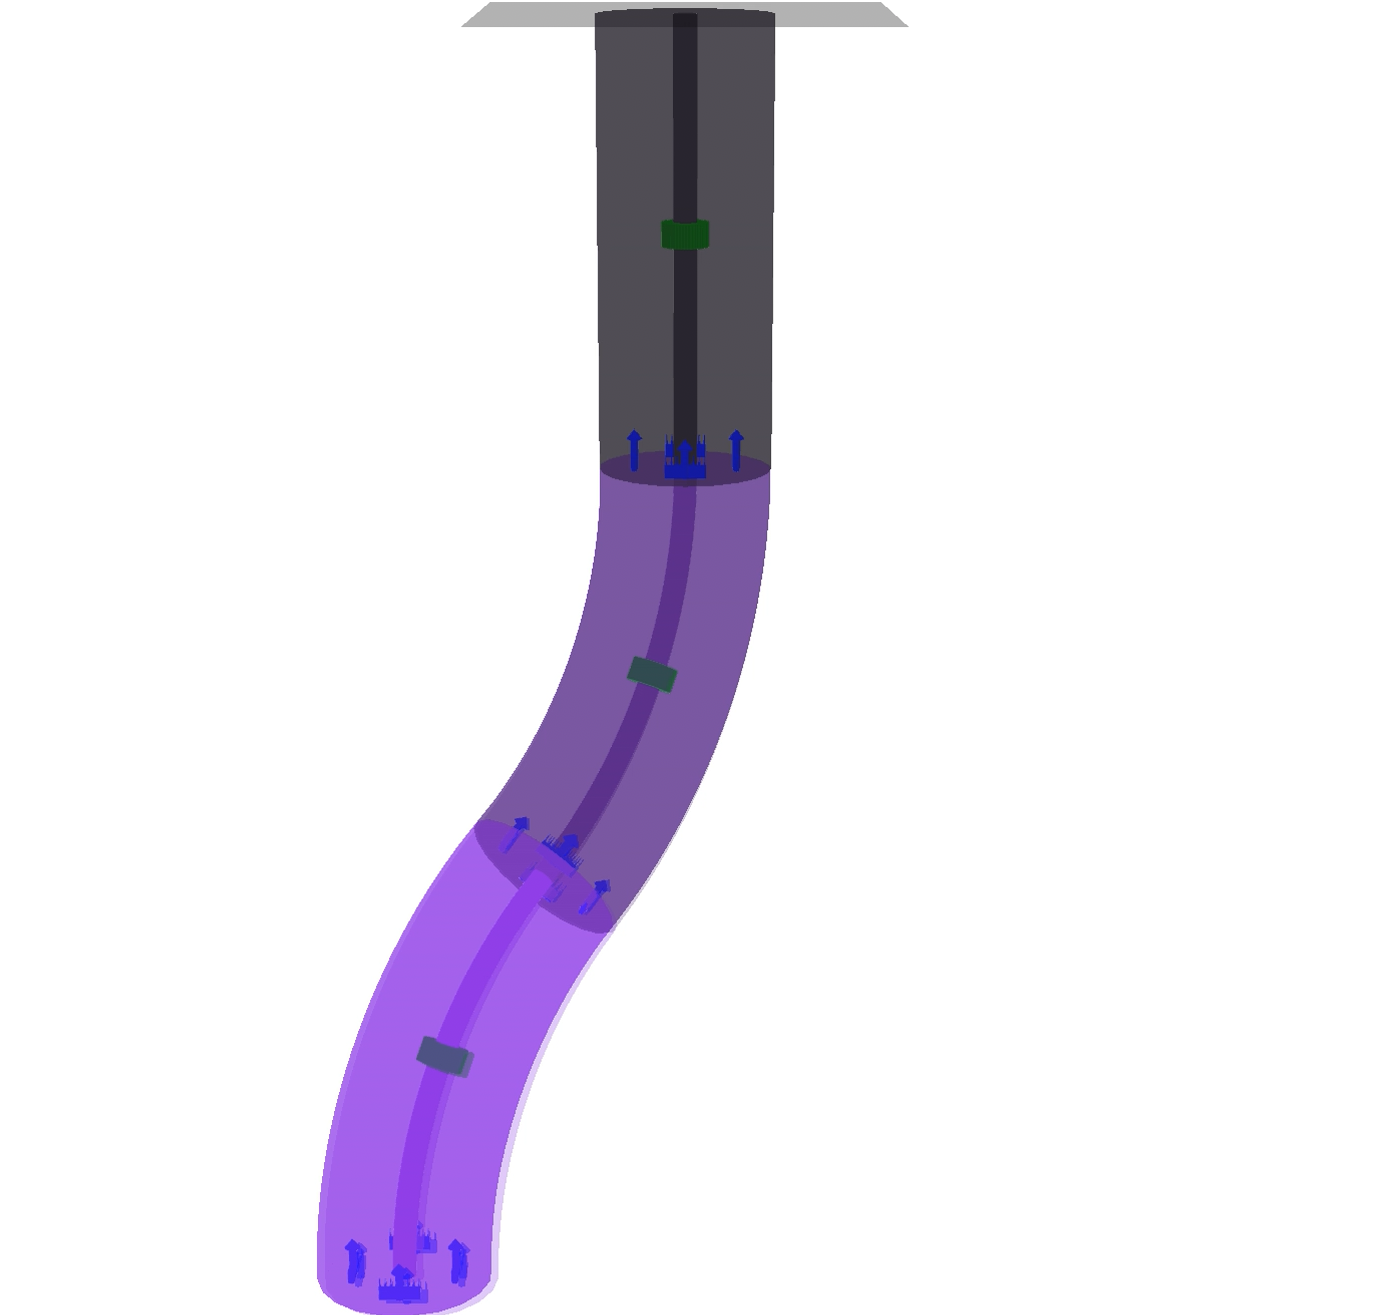
\includegraphics[width=0.161\textwidth]{promasens/figures/simulation_sequences/pcc_simulated_sensor_failure/simulated_sensor_failure_t=0s_cropped.png}}
  \hfill
  \subfigure[$t=\SI{2}{s}$]{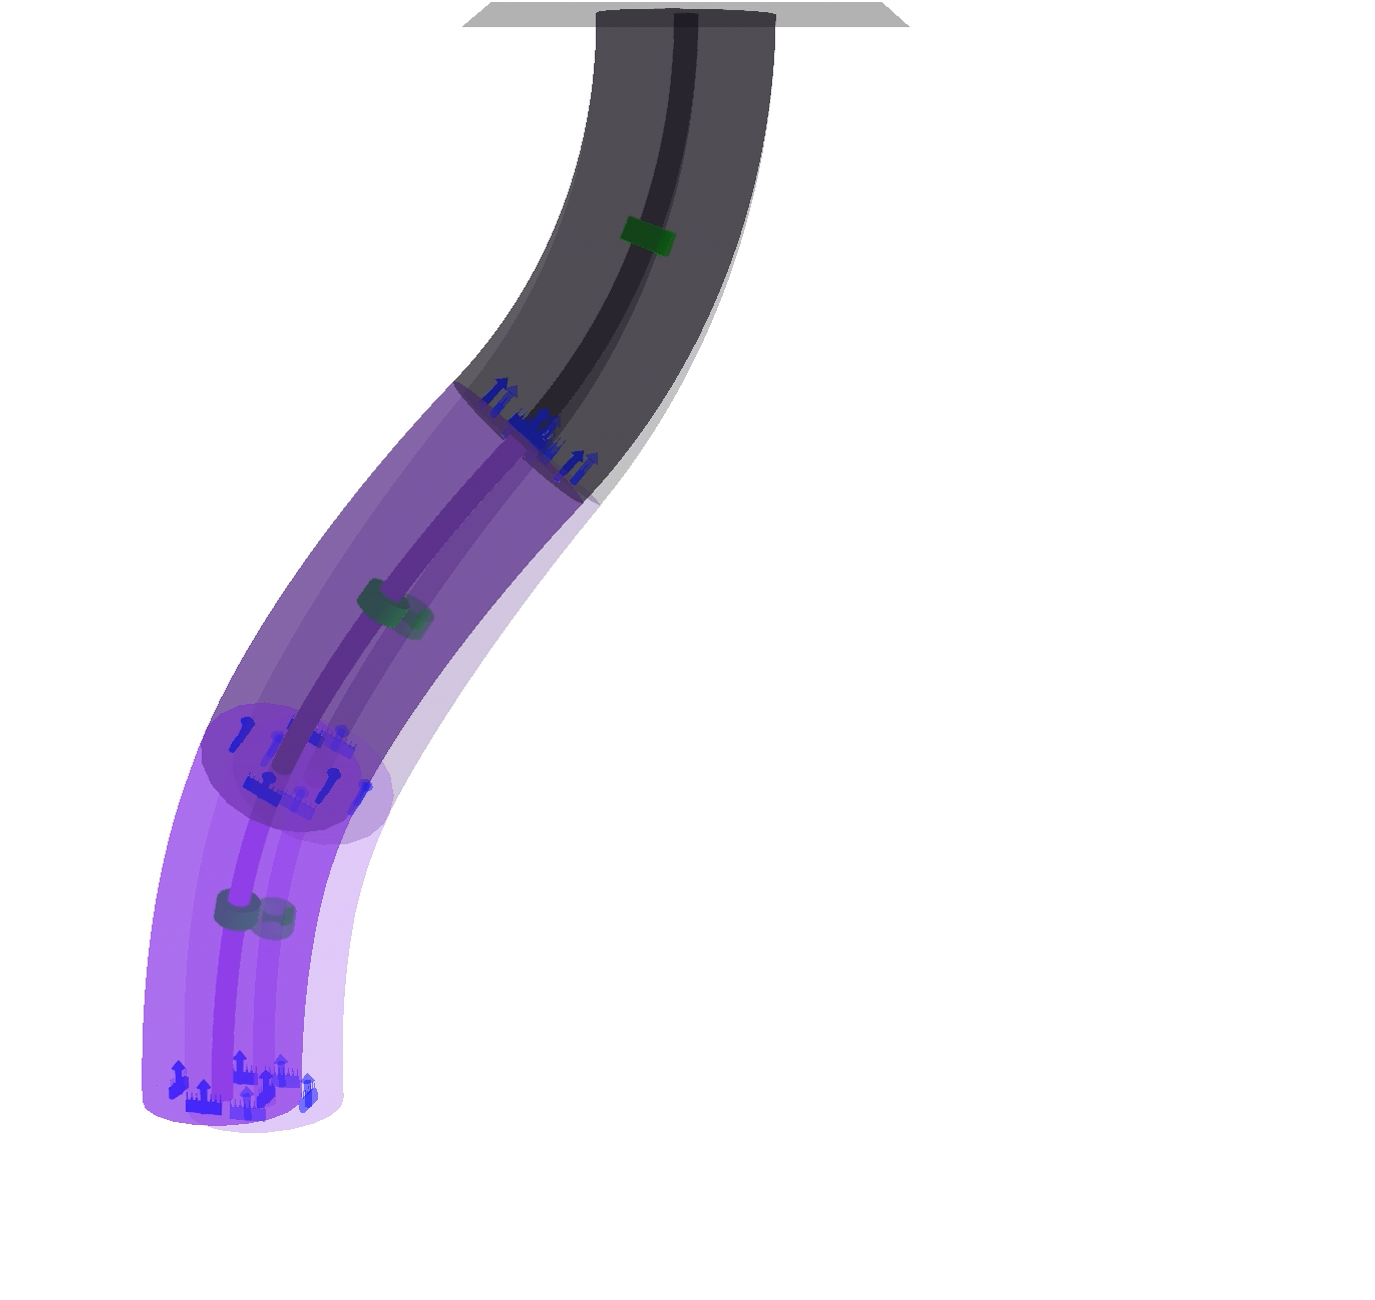
\includegraphics[width=0.161\textwidth]{promasens/figures/simulation_sequences/pcc_simulated_sensor_failure/simulated_sensor_failure_t=2s_cropped.png}}
  \hfill
  \subfigure[$t=\SI{4}{s}$]{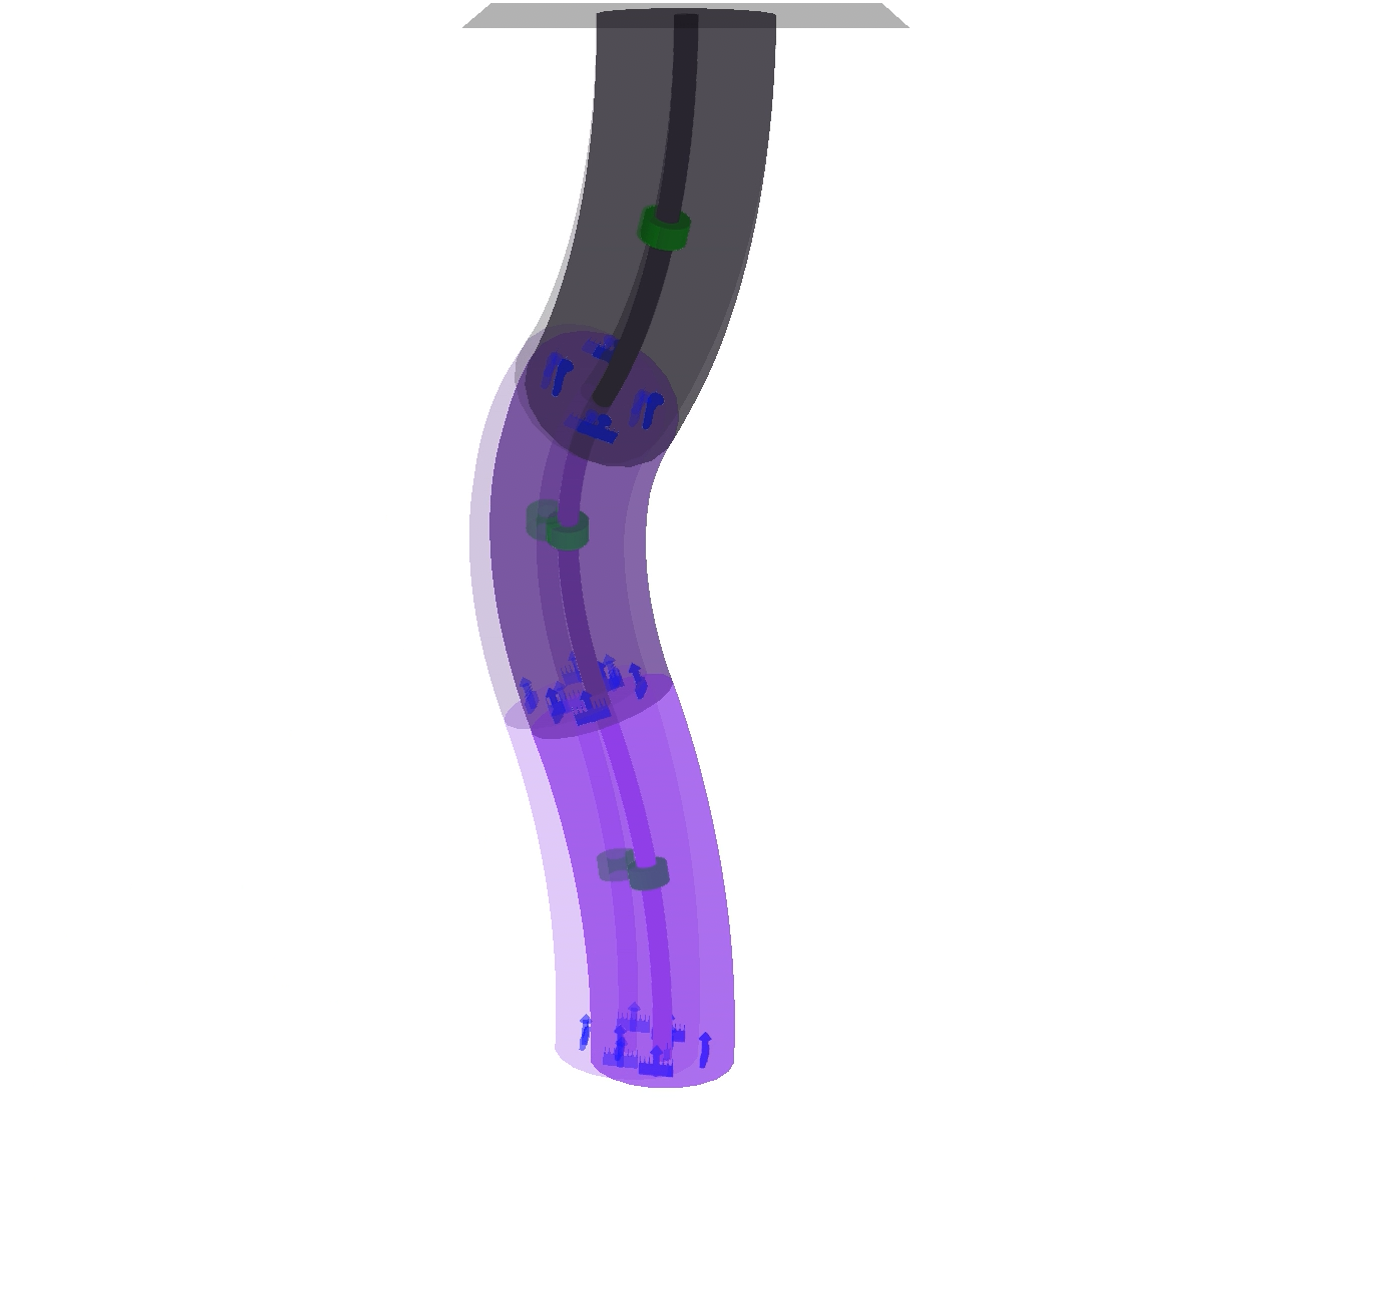
\includegraphics[width=0.161\textwidth]{promasens/figures/simulation_sequences/pcc_simulated_sensor_failure/simulated_sensor_failure_t=4s_cropped.png}}
  \hfill
  \subfigure[$t=\SI{6}{s}$]{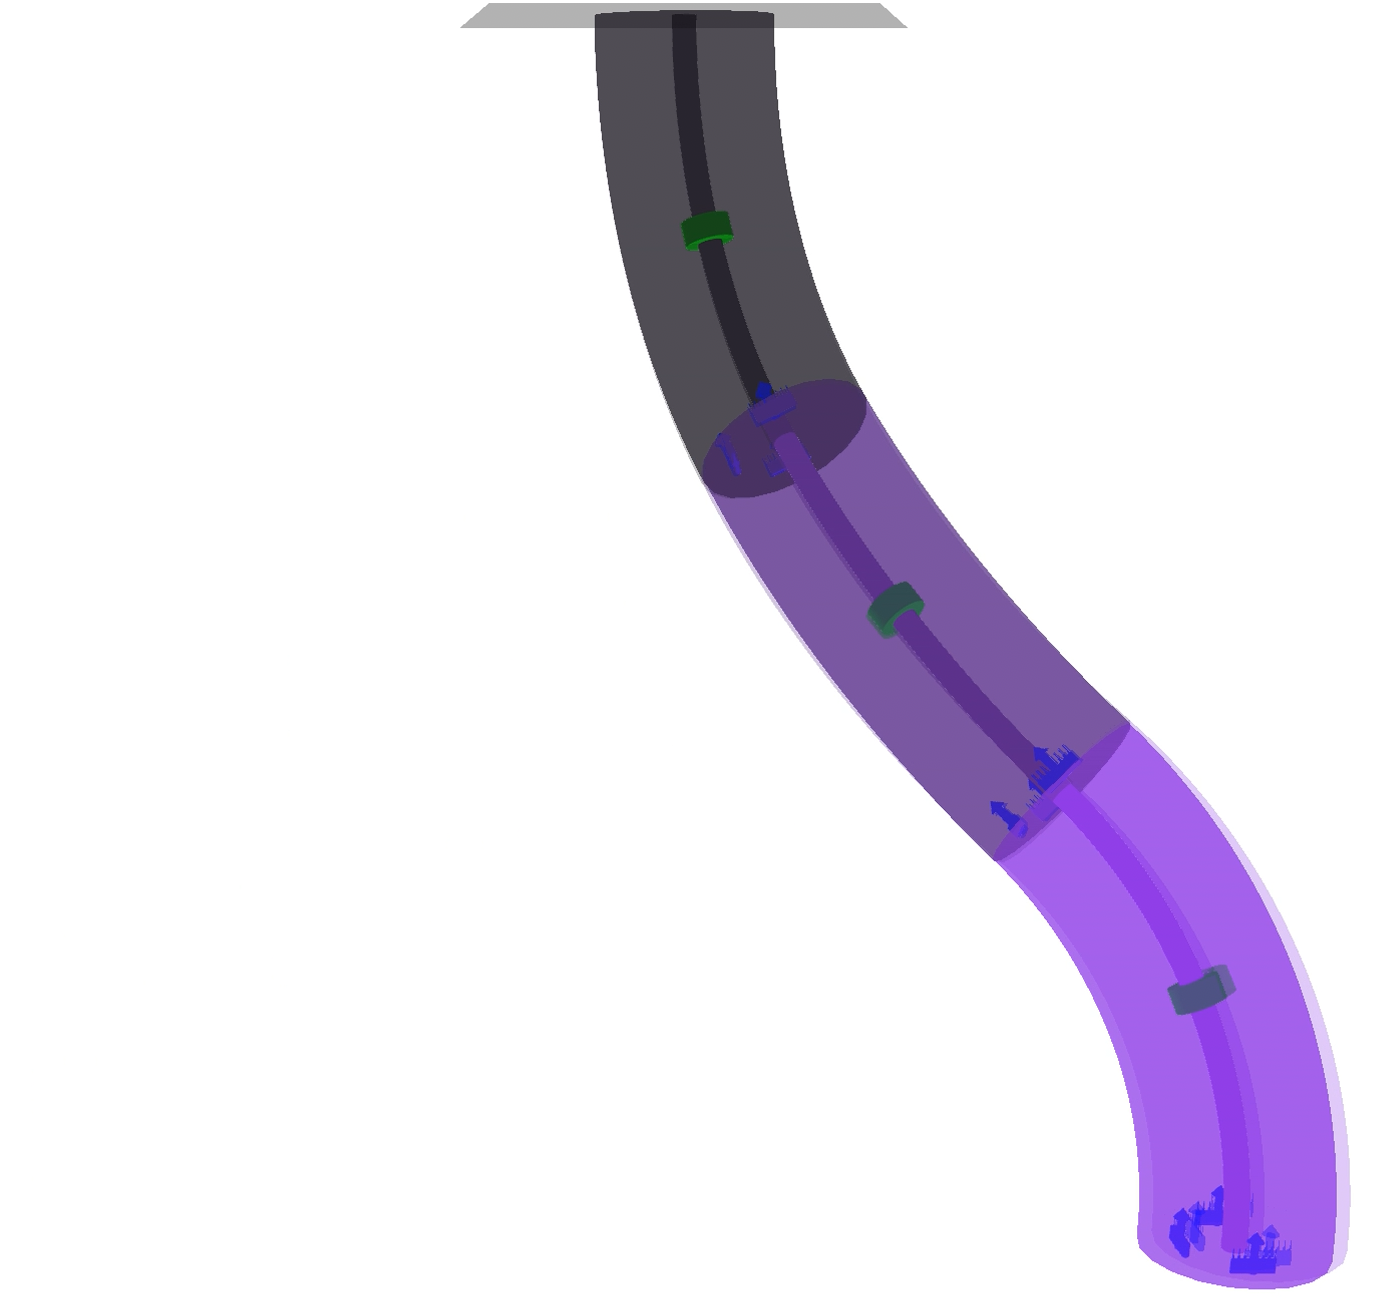
\includegraphics[width=0.161\textwidth]{promasens/figures/simulation_sequences/pcc_simulated_sensor_failure/simulated_sensor_failure_t=6s_cropped.png}}
  \hfill
  \subfigure[$t=\SI{8}{s}$]{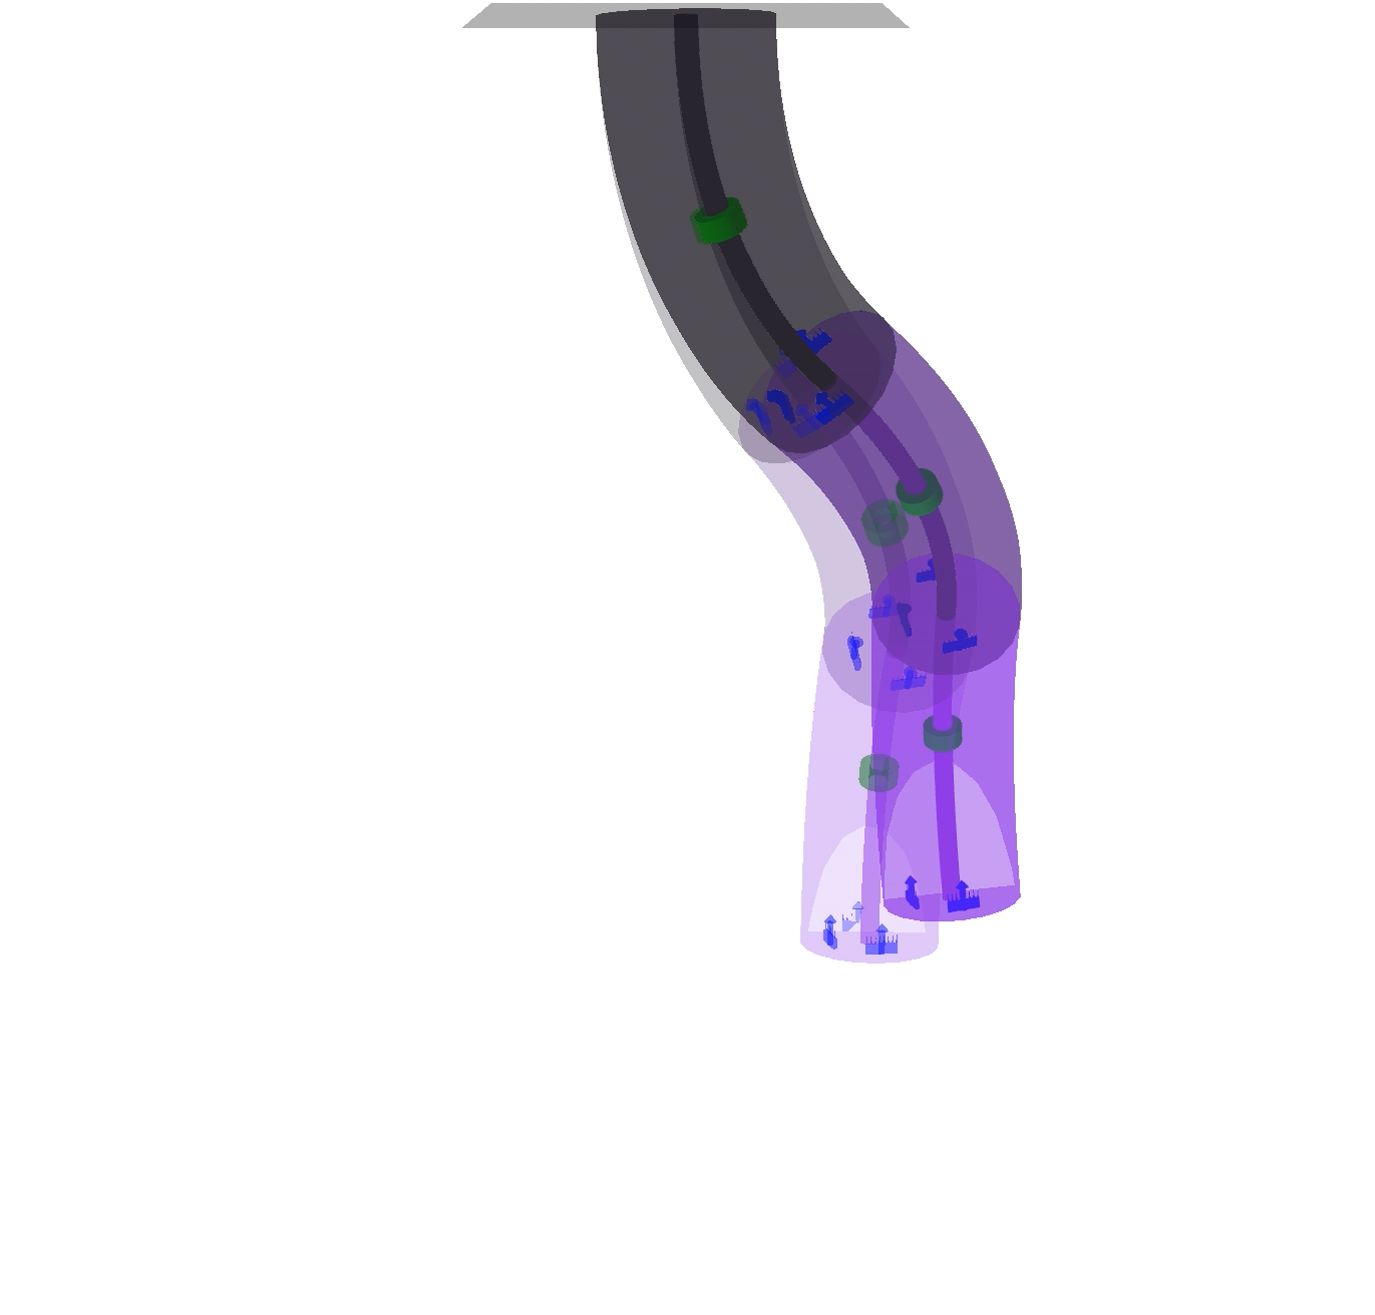
\includegraphics[width=0.161\textwidth]{promasens/figures/simulation_sequences/pcc_simulated_sensor_failure/simulated_sensor_failure_t=8s_cropped.png}}
  \hfill
  \subfigure[$t=\SI{10}{s}$]{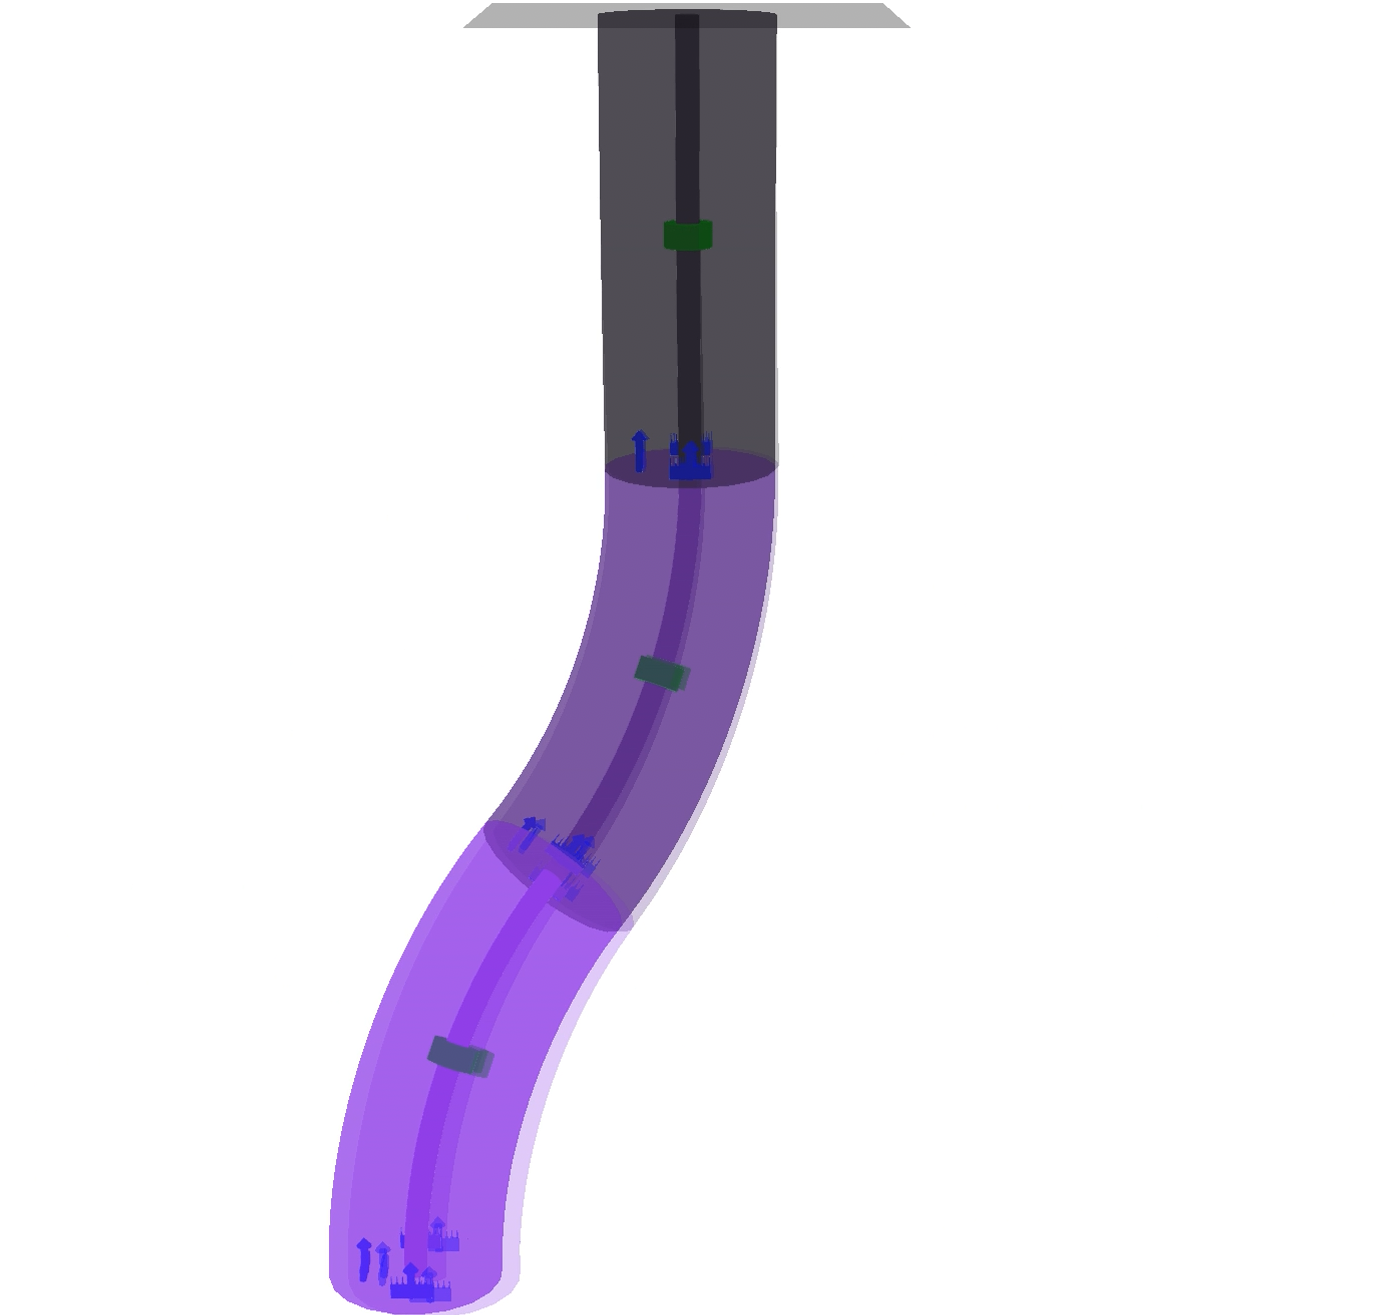
\includegraphics[width=0.161\textwidth]{promasens/figures/simulation_sequences/pcc_simulated_sensor_failure/simulated_sensor_failure_t=10s_cropped.png}}
  % 1375px x 1315px
  \caption{Sequence of stills for simulated sensor failure as shown in Figure~\ref{fig:promasens:simulated_sensor_failure}: the number of sensors per segment, which are rendered in blue, is reduced from four to three at $t=\SI{5}{s}$. We visualize the ground-truth shape of the soft robot with full opacity and the estimated configuration with slight transparency. The magnets are rendered in green and the three segments are visualized in a color sequence from black to violet.}
  \label{fig:promasens:simulation_sequences}
\end{figure*}

\subsection{Optimization}
We optimize the configuration variables $\hat{q}_i = (\hat{\Delta}_{x,i}, \hat{\Delta}_{y,i}, \hat{\delta} L_{i})^\mathrm{T}$ for each segment to minimize the sensor measurement prediction loss as defined in \eqref{eq:promasens:proprioception_loss}.
The optimization strategy solely relies on gradient descent and uses the best solution from the last time step $\hat{q}^*(t-1)$ as an initialization $\hat{q}_0(t)$. For the first time step of the trajectory, we initialize with the ground truth.
We use a step size $\gamma = 3.5 \cdot 10^{-4}$, $3 \cdot 10^{-3}$, and $2 \cdot 10^{-3}$ during gradient descent for a one-segment, two-segment and three-segment robot respectively. For all robots with more than one segment, the step size is reduced by a factor of ten when optimizing the elongation. The momentum $\mu$ is $0.3$ for all trials and we perform $20$ gradient descent iterations for each time step.

\subsection{Evaluation}\label{sub:promasens:pcc_simulations:evaluation}
We evaluate the performance of our method at estimating the configuration of the segment by computing a relative Root Mean-Squared Error (RMSE) metric with respect to the ground-truth configuration $q(t)$ for each configuration variable separately
\begin{equation}\label{eq:promasens:relative_RMSE}
\begin{split}
    e_{q_\star} = \frac{\sqrt{\sum_{t=0}^{n_\mathrm{t}} \left ( \hat{q}_\star(t) - q_\star(t) \right )^2}}{\sqrt{n_\mathrm{t}} \; D_{q_\star}},\\
    % e_{\Delta_y} = \frac{\sqrt{\sum_{t=0}^{n_\mathrm{t}} \left ( \hat{\Delta}_y(t) - \Delta_y(t) \right )^2}}{\sqrt{n_\mathrm{t}} \; L_{\Delta_y}},\\
    % e_{\delta L} = \frac{\sqrt{\sum_{t=0}^{n_\mathrm{t}} \left ( \delta \hat{L}(t) - \delta L(t) \right )^2}}{\sqrt{n_\mathrm{t}} \; L_{\delta L}},
\end{split}
\end{equation}
where $n_\mathrm{t}$ is the number of discrete time-steps and $D_{q_\star}$ is the dynamic range of each configuration variable between the maximum and minimum value in the test set.
All simulations are evaluated on a full lemniscate trajectory, which is very similar to what is plotted based on experimental data in Fig.~\ref{fig:promasens:t3_viz}. The maximum bending angle of this trajectory is \SI{45}{\degree} and the elongation of the segment follows a cosine wave with a minimum and maximum at \SI{1.25}{\percent} and \SI{3.75}{\percent} respectively.

\subsection{Results}\label{sub:promasens:simulation_pcc_results}
We present all simulation results in Tab.~\ref{tab:results_pcc_simulations}.
In the first section, robots with one to three segments, which all exhibit a nominal sensor placement, are considered separately. Neural networks are trained separately for each of these robots, as the input dimension needs to be adjusted to the number of magnets.
% We plot the configuration estimates for the three-segment robot in Fig.~\ref{fig:promasens:simulations_plot}.
The results show that the method works well for robots with 1-3 segments. It can be observed that the estimation error is usually lower for the distal segment(s).

Next, the number of sensors $n_\mathrm{s}$ is varied for a three-segment robot. We always apply a symmetrical placement of the sensors in the tip plane of each segment. In the first trial, two sensors are mounted in the tip plane of each segment opposite to each other (6 sensors in total). While the bending along $\Delta_{x,i}$ and the elongation of the segments $\delta L_i$ can still be estimated, the setup does not contain sufficient information to accurately determine the bending into $\Delta_{y,i}$.
While the nominal case of nine sensors in total already achieves relative RMSEs in the range of \SI{1.6}{\percent} to \SI{6}{\percent}, the proprioception performance can be slightly improved by adding more sensors.
% Recall that no re-training of the neural network is required when adding or removing sensors.
We emphasize that the neural networks are not retrained when adding or removing sensors.
In Figures~\ref{fig:promasens:simulated_sensor_failure} and \ref{fig:promasens:simulation_sequences}, we plot the proprioceptive performance of a three-segment robot with four sensors per segment. Then, we simulated a failure of the 4th, 8th, and 12th sensor at \SI{5}{s} by removing these sensor measurements from \eqref{eq:promasens:gradient_descent} (i.e. the gradient descent). Our method is able to adapt without re-training and leverage the nominal redundancy of sensor measurements, as three sensors per segment are sufficient for shape estimation.

Then, two adjusted sensor placements are investigated, while keeping the neural network weights constant. First, the sensors are tilted from the nominal case of pointing along the local z-axis by $\psi_\mathrm{s} = \SI{10}{\degree}$ towards the inside. In a separate simulation, the sensors are moved radially from nominally \SI{13}{mm} to \SI{16}{mm}. As the results show, the configuration of all three segments can still be estimated accurately with a mean error of \SI{3.3}{\percent}.

Finally, an earth's magnetic field of magnitude \SI{0.065}{mT} is added. A separate neural network is trained on a training set with randomly sampled magnetic field vector directions $n_\mathrm{e}$. As the last section of Tab.~\ref{tab:results_pcc_simulations} demonstrates, the methodology is able to adapt to any earth's magnetic field direction by leveraging the $\lambda_j$ input parameter.

% \subsection{Synthetic results}\label{sub:promasens:synthetic_results}
% We initially verify and quantitatively compare our method with an end-to-end trained neural network using a synthetic sensor measurement model: \textcolor{red}{Insert citation why we are using this synthetic sensor measurement model and also describe the \gls{NN} and how it differs from \gls{NN} from our method}
% \begin{equation}
%     u_j = \sum_{k=1}^{n_\mathrm{m}} \frac{1000}{d_{jk}^2} \cdot \cos( \theta_{jk}) \cdot \cos( \beta_{jk}) + n_u
% \end{equation}

% Alternatively, we implement a more realistic, analytical 2D model for the magnetic flux intensity of one magnet $k$ measured by sensor $j$. As our segment is axially symmetric, we can a 2D magnetic flux model in the plane of the angle $\theta_{jk}$. Referring to \eqref{eq:promasens:d_jk} and \eqref{eq:promasens:theta_jk}, we define the radial and axial distance between the magnet and the sensor as:
% \begin{equation}
%     d_{a,jk} = \cos(\theta_{jk}) \cdot d_{jk} \qquad d_{r,jk} = \sin(\theta_{jk}) \cdot d_{jk}
% \end{equation}
% For a magnet with thickness $h_m$ and of diameter $D_m$ in a medium with a relative magnetic permeability $\mu_o$ (for air $1.00000037$) and $M_a$ the surface magnetization magnitude of the magnet, we can define the magnetic field vector components in the cylindrical coordinate system of the magnet $jk$ as~\citep{furlani2001permanent, ozel2015precise}:
% \begin{equation}\scriptsize
% \begin{split}
%     B^a(d_a, d_r) = \frac{\mu_0 M_x}{2 \pi} \Bigg ( & \quad \arctan \frac{2 h_m \cdot (d_a + D_m)}{(d_a + D_m)^2 + d_r^2 - h_m^2} \\ 
%     & - \arctan \frac{2 h_m \cdot (d_a - D_m)}{(d_a - D_m)^2 + d_r^2 - h_m^2} \Bigg ),\\
%     B^r(d_a, d_r) = \frac{\mu_0 M_x}{2 \pi} \Bigg ( & \quad \ln \frac{(d_a + D_m)^2 + (d_r - h_m)^2 }{(d_a + D_m)^2 + (d_r + h_m)^2} \\ 
%     & - \ln \frac{(d_a - D_m)^2 + (d_r - h_m)^2 }{(d_a - D_m)^2 + (d_r + h_m)^2}  \Bigg ).
% \end{split}
% \end{equation}
% We rotate the translation between the magnet and the sensor into the magnet frame $\{S_{\mathrm{m}_k}\}$ and project it into the local x-y plane:
% \begin{equation}
%     t_{\mathrm{m}_k,xy}^{jk} = 
%     \mathrm{diag}(\begin{bmatrix} 1 & 1 & 0 \end{bmatrix}) 
%     \cdot (R_{i-1}^{\mathrm{m}_k})^{\mathrm{T}} \cdot t_{i-1}^{jk},
% \end{equation}
% which allows us to define the magnetic field vector in the frame $\{ S_{\mathrm{m}_k} \}$:
% \begin{equation}
%     B_{\mathrm{m}_k}^{jk} = 
%     \begin{bmatrix}
%         \frac{x^{t_{jk}}_{\mathrm{m}_k,xy}}{\lVert  t_{\mathrm{m}_k,xy}^{jk} \rVert} \cdot B^{r,jk} & \frac{y^{t_{jk}}_{\mathrm{m}_k,xy}}{\lVert  t_{\mathrm{m}_k,xy}^{jk} \rVert} \cdot B^{r,jk} & B^{a,jk}
%     \end{bmatrix}^{\mathrm{T}}.
% \end{equation}
% Next, we compute the expected sensor measurement $u_j$ using the scalar projection of the magnetic field vector $B_{i-1}^{jk}$ along the sensor measurement unit vector $\{ \hat{o}_{\mathrm{s}_j} \}_{i-1}$ with the dot product as:
% \begin{equation}
%     u_j = \sum_{k=1}^{n_\mathrm{m}} \left ( R_{i-1}^{\mathrm{m}_k} \cdot B_{\mathrm{m}_k}^{jk} \right ) \cdot \{ \hat{o}_{\mathrm{s}_j} \}_{i-1}
% \end{equation}

% We apply both input and process Gaussian noise to pose a realistic challenge for both proprioception methods.
% \textcolor{red}{Please insert the correct noise values here:}
% We add the process noise $n_u \sim \mathcal{N}\left(\SI{0.2}{V}, \SI{0.5}{V} \right)$ to the target sensor measurement $u$ and the inputs noise $n_d \sim \mathcal{N}\left(\SI{0.2}{m}, \SI{0.5}{m} \right)$, $n_\theta \sim \mathcal{N}\left(\SI{0.2}{\degree}, \SI{0.5}{\degree} \right)$ and $n_\beta \sim \mathcal{N}\left(\SI{0.2}{\degree}, \SI{0.5}{\degree} \right)$ before $\Bar{\xi}$ is passed to the neural network:
% \begin{equation}
%     \Bar{\xi}_{jk} = \xi_{jk} + 
%     \begin{bmatrix}
%     n_d & n_\theta & n_\beta
%     \end{bmatrix}^\mathrm{T}
% \end{equation}
